\documentclass[a4paper, 12pt, twoside, openright]{book}
\addtolength{\oddsidemargin}{+1.3cm}
\addtolength{\evensidemargin}{-1.3cm}
\usepackage[english]{babel}
\usepackage[T1]{fontenc}
\usepackage[utf8]{inputenc}
\usepackage{fancyhdr}
\usepackage{float}
\usepackage{graphicx}
\usepackage{wrapfig}
\usepackage{siunitx} %per scrivere il simbolo °
\usepackage{verbatim} %per i commenti1
\usepackage{subcaption}
\usepackage{amsmath}
\usepackage{algorithm}
\usepackage{algpseudocode}
\setcounter{secnumdepth}{3}
\setcounter{tocdepth}{6}
\usepackage{multirow}
\usepackage{enumitem}
\newcommand{\minitab}[2][l]{\begin{tabular}#1 #2\end{tabular}}
\usepackage{rotating}
\usepackage{url}
\newlist{tabitem}{itemize}{1}
\setlist[tabitem]{wide=0pt, nosep, leftmargin= * ,label=\textbullet,after=\vspace{-\baselineskip},before=\vspace{-0.6\baselineskip}}

\DeclareMathOperator*{\argmax}{arg\,max}
\DeclareMathOperator*{\argmin}{arg\,min}

%\usepackage{booktabs,array}
%\usepackage{tikz}

%\usepackage{tabularx}

%\usepackage{chngcntr}
%\counterwithin{table}{section}

%------------------------------ colors
\usepackage[usenames,dvipsnames,table]{xcolor} % use colors on table and more
\definecolor{333}{RGB}{51, 51, 51} % define custom color
\definecolor{background}{RGB}{255, 254, 213}
\definecolor{comment}{RGB}{17,167,5}
\definecolor{keyword}{RGB}{195,47,8}
\definecolor{string}{RGB}{142,195,0}
\definecolor{number}{RGB}{90,84,84}
\definecolor{identifier}{RGB}{0,90,201}

%------------------------------ source code
\usepackage{listings}

\lstset{
  basicstyle=\footnotesize\sffamily,
  commentstyle=\itshape\color{gray},
  captionpos=b,
  frame=shadowbox,
  language=HTML,
  rulesepcolor=\color{333},
  tabsize=2
}

\lstdefinestyle{code}{
  backgroundcolor=\color{background},
  basicstyle=\footnotesize\sffamily,
  commentstyle=\color{comment},
  frame=L,
  identifierstyle=\color{identifier},
  keywordstyle=\color{keyword},
  numbers=left,
  numbersep=10pt,
  numberstyle=\tiny\color{number},
  stringstyle=\color{string},
  showstringspaces=false,  
  stepnumber=1,
  tabsize=2
}

\usepackage[colorlinks=true, linkcolor=black, citecolor=blue, urlcolor=black]{hyperref}

%------------------------------ define Abstract environment, missing in the 'book' class
\newenvironment{abstract}{\cleardoublepage \null \vfill \begin{center}\bfseries\abstractname \end{center}}{\vfill\null}
\addto\captionsenglish{\renewcommand*\abstractname{Abstract}} % change Abstract title

%------------------------------ active url
\usepackage{url}
\renewcommand{\UrlFont}{\color{black}\small\ttfamily} % active ref
%------------------------------ macros
\newcommand{\sectionname}{Section} % define Section ref
\newcommand{\subsectionname}{Sub-section} % define Sub-section ref
\renewcommand*\arraystretch{1.4} % tables padding

%acronimi
\usepackage[printonlyused]{acronym}

%Formatted quote
\newcommand{\myquote}[2]{
\begin{quote}
	\textbf{\Large ``}{\textit{#1}}\textbf{\Large ''}\\
	\textbf{#2}\\\\
\end{quote}
}

%Formatted item with description
\newcommand{\descItem}[2]{
\item{\textbf{#1}\\#2}
}

\begin{document}
\frontmatter
\begin{titlepage} %------------------------------ TITLE PAGE
\begin{center}
\vbox to0pt{\vbox to\textheight{\vfill 
\includegraphics[width=11.5cm]{./Images/unipd-light} \vfill}\vss}

\begin{minipage}{.20\textwidth}
  
\includegraphics[height=2.5cm]{./Images/unipd-bn}
\end{minipage}\begin{minipage}{.90\textwidth}
  \begin{table}[H]
  \begin{tabular}{l}
  \scshape{\Large{\bfseries{University of Padova}}} \\
  \hline
  \scshape{\Large{Engineering~Departement}} \\
  \end{tabular}
  \end{table}
\end{minipage}

\vspace{1cm}
\emph{\Large{Computer~Engineering~Master~Degree}} \\
\vspace{1.5cm}
\scshape{\Large{\bfseries{AcCAPPCHA:\\}}}
\scshape{\large{\bfseries{Design, Development and Security Analysis\\}}}
\scshape{\large{\bfseries{of an Invisible CAPPCHA based on\\}}}
\scshape{\large{\bfseries{an acoustic side-channel\\}}}
\vspace{0.2cm} \linespread{1} 
\scshape{\large{\bfseries{}}}
\end{center}

\vfill
\begin{normalsize}
\begin{flushleft}
  %\hspace{45pt} \textit{Laureando} \hspace{160pt} \textit{Relatore}\\
  \hspace{65pt} \textit{Candidate} \hspace{130pt} \textit{Supervisor}\\
  \vspace{5pt}
  \hspace{25pt} \large{\textbf{\footnotesize{Di Nardo Di Maio Raffaele}}} \hspace{55pt} \large{\textbf{\footnotesize{Prof. Migliardi Mauro}}}\\
\end{flushleft}
\end{normalsize}

\vfill
\begin{center}
\textsc{DD-MM-2021}
\hspace{-0.2cm}
\line(1, 0){360}

\textsc{Accademic Year 2021-2022}
\end{center}
\end{titlepage}
\cleardoublepage % make left page blank
\thispagestyle{empty}
\null
\vspace{2cm}
\begin{flushright}
     To my parents, who always help\\
   me to be happy doing what I love\\
and support me in reaching my goals.
\end{flushright}
\vfill
\cleardoublepage % make left page blank
\null
\vspace{2cm}
\thispagestyle{empty}
\myquote{Most people assume that once security software is installed, they're protected. This isn't the case. It's critical that companies be proactive in thinking about security on a long-term basis.}{Kevin Mitnick}
\myquote{You have to learn the rules of the game. And then you have to play better than anyone else.}{Albert Einstein}
\myquote{Si come il ferro s'arrugginisce sanza esercizio, e l'acqua si putrefà o nel freddo s'addiaccia, così lo 'ngegno sanza esercizio si guasta.}{Leonardo da Vinci}
\vfill
\null
%\begin{abstract} %------------------------------ ABSTRACT
%\addcontentsline{toc}{chapter}{Abstract}
%\markboth{}{} % remove header
%\thispagestyle{empty}
%This is the abstract
%\end{abstract}

%%\begin{abstract} %------------------------------ ABSTRACT
%\addcontentsline{toc}{chapter}{Abstract}
%\markboth{}{} % remove header
%\thispagestyle{empty}
%This is the abstract
%\end{abstract}

%%\begin{abstract} %------------------------------ ABSTRACT
%\addcontentsline{toc}{chapter}{Abstract}
%\markboth{}{} % remove header
%\thispagestyle{empty}
%This is the abstract
%\end{abstract}

%\input{Chapters/Abstract.tex}

\begingroup %------------------------------ CONTENTS
  \makeatletter
  \let\ps@plain\ps@empty
  \makeatother
  \tableofcontents  
  \clearpage
\endgroup

\mainmatter
\chapter{Introduction}
\begin{itemize}
\item{\textbf{Arithmetic}\\
}
\item{\textbf{Audio-based}\\
}
\item{\textbf{Game-based}\\
}
\item{\textbf{Image-based}\\
}
\item{\textbf{Puzzle-based}\\
}
\item{\textbf{Text-based}\\
}
\item{\textbf{Video-based}\\
}
\end{itemize}

\begin{table}
\centering \footnotesize
\renewcommand*\arraystretch{1.3}
\begin{tabular}{cll}
\hline
{\textbf{CAPTCHA type}} & {\textbf{Usability issues}} & {\textbf{Security}}\\
\hline
\textit{Arithmetic} & {} & {}\\
\hline
\textit{Audio-based} & {
  \begin{minipage} [t] {0.4\textwidth}
  Issues of recognition:
      \begin{itemize}
        \item{Previous knowledge of English dictionary by the user.}
        \item{Some character sounds very similar to others.}
       \end{itemize} 
  \end{minipage}
} & {}\\
\tabularnewline
\hline
\textit{Game-based} & {} & {}\\
\hline
\textit{Image-based} & {
 \begin{minipage} [t] {0.4\textwidth}
Difficulty of identification of images caused by:
      \begin{itemize}
        \item{Blur of images.}
        \item{Low vision condition.}
       \end{itemize} 
  \end{minipage}
} & {}\\
\tabularnewline
\hline
\multirow{2}{*}{\textit{Puzzle-based}} & {It takes too much time to solve the puzzle} & {}\\
{} & {and to identify the arrangement of puzzles.} & {}\\
\hline
\textit{Text-based} & {
  \begin{minipage} [t] {0.4\textwidth}
	Many problems have to be solved by user:
      \begin{itemize}
        \item{Multiple fonts.}
        \item{Font size.}
        \item{Blurred Letters}
        \item{Wave Motion.}
       \end{itemize} 
  \end{minipage}
}
& {It can be identified by OCR (Optical Character Recognition) technique.}\\
\tabularnewline
\hline
\textit{Video-based} & {
Issues downloading videos to find correct} & {}\\
{} & {captcha because of large size of files.} & {}\\

\end{tabular}
\end{table}
\chapter{State of the Art}\label{chapter:StateOfArt}
CAPTCHA is the acronym of \textit{"Completely Automated Public Turing-test-to-tell Computers and Humans Apart"} and it's a challenge born from these two components\cite{types_CAPTCHA}:
\begin{enumerate}
\descItem{Human-Computer Interaction (HCI)}
{it is a research field that studies the computer technology, looking at the interfaces between the users and the machines. A human can interact with a machine at several levels:
\begin{itemize}
	\item{Task level}
	\item{Semantic level}
	\item{Syntactic level}
	\item{Interactive level}
	\item{Physical devices level}
\end{itemize}
This discipline tries to analyse the ways in which a human can process data, matching the user's needs and interests. According to cognitive psychology studies, the human interaction with the machine is based on:
\begin{itemize}
	\item{Reasoning}
	\item{Problem solving}
	\item{Skill acquisition}
	\item{Error}
\end{itemize}   
}
\descItem{Human Interactive Proof (HIP)}
{it's a proof used to classify machines and humans looking at a specific type of interaction, that is simple to be done by a human instead of a bot. The main goals of the test are:
\begin{itemize}
	\item{To differentiate the humans from the computers}
	\item{To differentiate a category of the humans}
	\item{To differentiate a specific human from the category of humans}
\end{itemize}
HIP consists of a test program administered to humans and computers. The main problem of this proof is that the complexity of the task is often very complex and only a specific group of humans can usually solve the test.\\
Historically the most widely known version is the cognitive one defined by Alan Turing. The Turing test is used to determine how much a machine is capable of thinking like a human. The experiment involves three figures: a human examiner, a human and a machine. The examiner asks some questions to the other figures and, after a fixed amount of time, he evaluates if the two answers were different or not.\\
If they were similar, with respect to the point of view of the examiner, the machine is classified as an AI (Artificial Intelligence). The test is very reliable if each question could have many possible answers.}
\end{enumerate}
The design of CAPTCHA challenges takes inspiration from the previous components because its goal is to establish if the user is a bot or a human. A bot is usually an advanced program that exploits some AI techniques and pretends to be a human. In the endeavor of foiling bots that are getting every day smarter and more sophisticated, a CAPTCHA challenge sometimes is so complex that a human user can't solve it. For this reason and in order to guarantee an high level of security, a CAPTCHA has to satisfy the following requirements:
\begin{itemize}
	\item{There exists only one solution of a CAPTCHA and it shouldn't depend on the user's language and/or age;}
	\item{The solution of a CAPTCHA must be easy for the humans and hard for the bots. In fact humans should solve it in no longer than 30 seconds with very high success rate (30 seconds are usually considered too much time to solve a CAPTCHA);}
	\item{The creation of a CAPTCHA shouldn't affect the user privacy.}
\end{itemize}
Over the year, the CAPTCHAs must satisfy more and more requirements and the challenges become more and more complex reducing the usability of them. For this reason, a new generation of CAPTCHAs, that we define modern CAPTCHAs, has been developed in the last years. The new challenges are related to a good exploitation of the biometrics and the sensors of modern devices. In addition, machine learning techniques and side-channel information are used to evaluate the user behaviour instead of generating challenges based on cognitive capabilities. 

%\vspace{4cm}
\section{Traditional CAPTCHAs}
The traditional CAPTCHAs are based on the knowledge and the correct insertion of the solution by the user. These CAPTCHA schemes are designed to leverage character recognition, image analysis and speech recognition to guarantee that the challenges will successfully block bots.\\
The main types of traditional CAPTCHAs, namely Audio-based CAPTCHAs, Game-based CAPTCHAs, Image-based CAPTCHAs, Math CAPTCHAs, Slider CAPTCHAs, Text-based CAPTCHAs and Video-based CAPTCHAs, are described in the following sections but the details about specific implementations can be found in the article of Walid Khalifa Abdullah Hasan\cite{survey_advanced_CAPTCHA}. With respect to user experience, the most enjoyable traditional CAPTCHAs are usually the game-based and image-based ones while the most frustrating CAPTCHA is the text-based one\cite{usability_CAPTCHA}. A summary of usability and security issues, explained in the following sections, is also reported in \myref{Table}{soa:traditional_table}.

\subsection{Audio-based CAPTCHAs}
This type of CAPTCHAs asks the user to type the words contained in an audio file (see \myref{Figure}{soa:audio_CAPTCHA}). It's developed for vision-impaired users. Audio-based CAPTCHAs usually have problems in usability related to the language dictionary, from which the words are taken, and the similarity of sound for several words. This CAPTCHA is a hard task even for blind users, in fact  during an experiment only 46\% of the challenges were solved by the participants\cite{usability_audio}.\\
One of the most popular Audio-Based CAPTCHAs is \textit{Audio reCAPTCHA}, developed at Carnegie Mellon University and then bought by Google. In this scheme, the user needs to recognize and write a set of 8 spoken characters from a noisy audio file with several background voices. If the user makes a mistake, the test declares that he's a bot.\\
Audio-based CAPTCHAs are vulnerable to many Automatic Speech Recognition (ASR) programs\cite{improving_audio} but also Deep Learning techniques (e.g. DeepCRACk\cite{DeepCRACk}). A good overview about results, obtained by several classification methods, is described in the work of Jennifer Tam et al.\cite{break_audio}.
\begin{figure}[h]
     \centering
     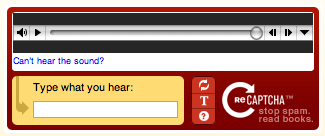
\includegraphics[width=.4\linewidth]{Images/StateOfArt/audio_CAPTCHA}
     \caption{\footnotesize{Example of audio-based CAPTCHA.}}\label{soa:audio_CAPTCHA}
\end{figure}

\subsection{Game-based CAPTCHAs}
This type of CAPTCHAs performs the verification of the user identity through a set of several kinds of games (see \myref{Figure}{soa:game}). The strength of Game-based CAPTCHAs is related to the the rules of the game that only humans can understand.\\
There exists an implementation of these CAPTCHAs, called \textit{Dynamic Cognitive Game (DCG)}, that is usually developed using Flash, HTML5 and JavaScript. These technologies download the game code to the client and execute it locally.\\
The code of these challenges must be the obfuscated to prevent that the source file could be analysed by an attacker. In fact, the obfuscation guarantees that the source code can not be stored on different internet domains. However for example, there exists a bot attack, called \textit{Stream Relay Attack}, that obtains good results bypassing these challenges \cite{game_CAPTCHA} (see \myref{Section}{soa:security_CAPTCHAs}).
\begin{figure}[h]
     \centering
     \begin{subfigure}[b]{0.48\textwidth}
         \centering
         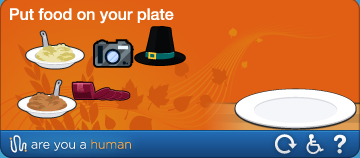
\includegraphics[width=.9\linewidth]{Images/StateOfArt/game_CAPTCHA}
     \end{subfigure}
     \hfill
     \begin{subfigure}[b]{0.48\textwidth}
         \centering
         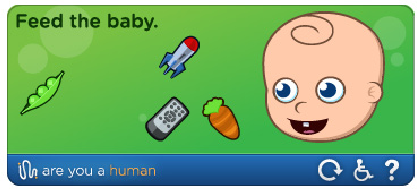
\includegraphics[width=.9\linewidth]{Images/StateOfArt/game_CAPTCHA2}
     \end{subfigure}
		
	 \begin{subfigure}[b]{0.55\textwidth}
         \centering
         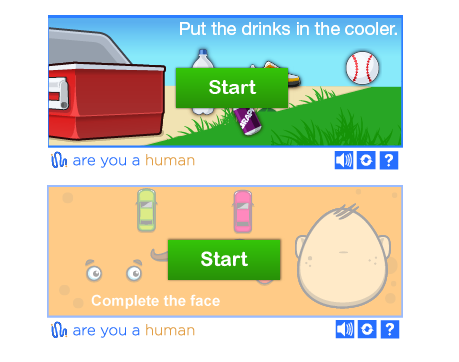
\includegraphics[width=\linewidth]{Images/StateOfArt/game_CAPTCHA3}
     \end{subfigure}
     \caption{\footnotesize{Examples of game-based CAPTCHAs.}}
     \label{soa:game}
\end{figure}

\subsection{Image-based CAPTCHAs}
Image-based CAPTCHAs is based on a written text that describes a task related to the evaluation of some images. The user must understand the action and he passes the test if he performs it in the right way. This type of CAPTCHAs can be categorized into the following classes, looking at the task that the user needs to perform:
\begin{itemize}
\descItem{Click-based CAPTCHAs}
{this type of CAPTCHAs shows an image and a text that explains where the user needs to click (see \myref{Figure}{soa:click_CAPTCHA}).
\begin{figure}[h]
     \centering
     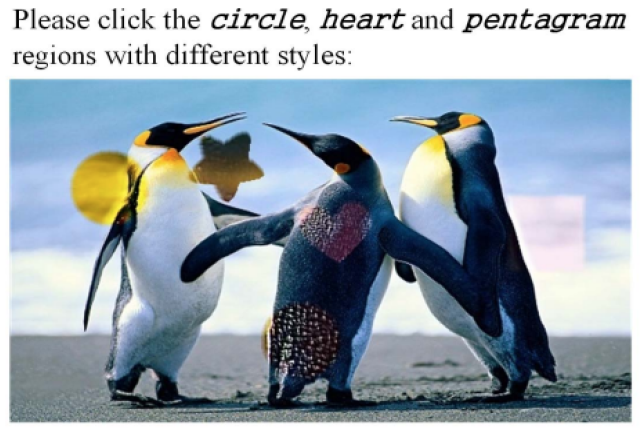
\includegraphics[width=.45\linewidth]{Images/StateOfArt/click_CAPTCHA}
     \caption{\footnotesize{Example of click-based CAPTCHA.}}\label{soa:click_CAPTCHA}
\end{figure}
}
\descItem{Sliding image-based CAPTCHAs}
{this type of CAPTCHAs asks the user to use the slider to solve an image-based challenge such as adjusting the orientation of an image, selecting the correct form of an image, or moving a fragment of an image to the correct location (see \myref{Figure}{soa:sliding_image}).
\begin{figure}[h]
     \centering
     \begin{subfigure}[b]{0.48\textwidth}
         \centering
         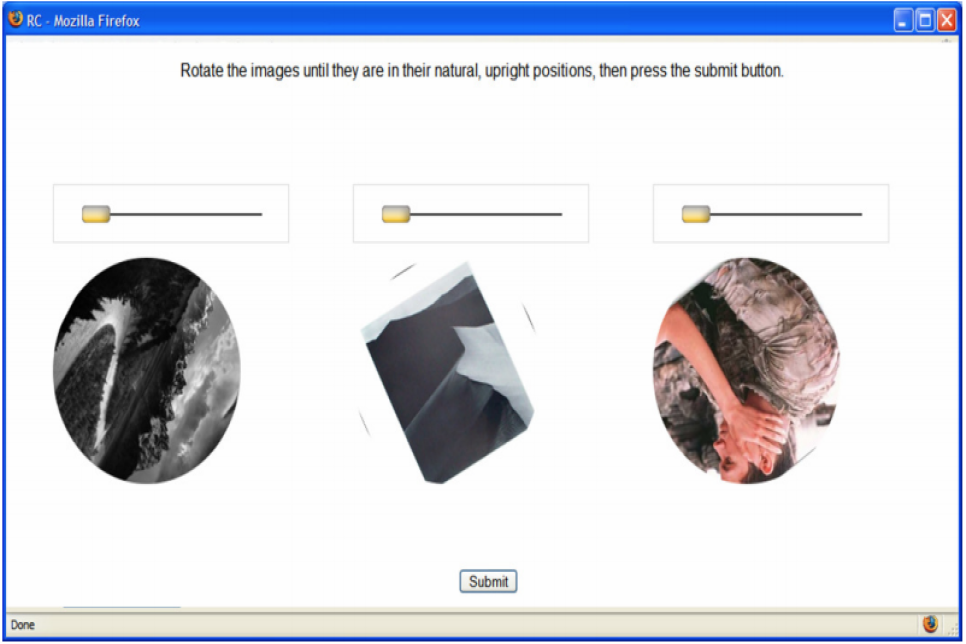
\includegraphics[width=.9\linewidth]{Images/StateOfArt/sliding_image_CAPTCHA}
	     \caption{\footnotesize{Orientation based.}}
     \end{subfigure}
     \hfill
     \begin{subfigure}[b]{0.48\textwidth}
         \centering
         
\includegraphics[width=.9\linewidth]{Images/StateOfArt/sliding_image_CAPTCHA2}
	     \caption{\footnotesize{Form based.}}
     \end{subfigure}
     \caption{\footnotesize{Examples of sliding image-based CAPTCHAs.}}
     \label{soa:sliding_image}
\end{figure}
}
\descItem{Drag \& Drop-based CAPTCHAs}
{this type of CAPTCHAs usually asks the user to complete a visual puzzle, created by dividing a given image in a set of pieces\cite{survey_CAPTCHA} (see \myref{Figure}{soa:puzzle}).\\
The task isn't easy for users because this type of CAPTCHAs takes more time to solve the puzzle but the security level is very high\cite{survey_CAPTCHA}. To improve the usability of the CAPTCHA, there exists a version of the puzzle-based CAPTCHA in which the user needs to insert only some pieces of the puzzle instead to complete it (see \myref{Figure}{soa:puzzle2}).
\begin{figure}[h]
     \centering
     \begin{subfigure}[b]{0.48\textwidth}
         \centering
         
\includegraphics[width=.6\linewidth]{Images/StateOfArt/puzzle_CAPTCHA}
         \caption{\footnotesize{Completing the puzzle.}}
         \label{soa:puzzle}
     \end{subfigure}
     \hfill
     \begin{subfigure}[b]{0.48\textwidth}
         \centering
         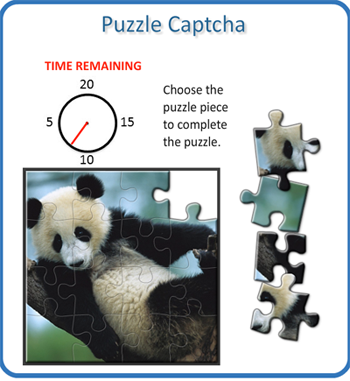
\includegraphics[width=.6\linewidth]{Images/StateOfArt/puzzle_CAPTCHA2}
         \caption{\footnotesize{Inserting only some pieces.}}
        \label{soa:puzzle2}
     \end{subfigure}
     \caption{\footnotesize{Examples of puzzle-based CAPTCHAs.}}
\end{figure}
}
\descItem{Selection-based CAPTCHAs}
{the user usually needs to select the images that contain a requested subject. The set of images, on which the user needs to identify the subject, can be created in several ways, for example:
\begin{itemize}
\item{An image is divided into a set of sub-squares and each of them is a candidate image (see \myref{Figure}{soa:selection})}
\item{There are many images, each one with a unique different subject (see \myref{Figure}{soa:selection2})}
\end{itemize}
This type of CAPTCHAs is vulnerable to different Object Recognition techniques developed for Computer Vision purposes.\\
An extension of this type of CAPTCHAs, called \textit{FaceDCAPTCHA}, has been introduced\cite{FaceDCAPTCHA} and it incorporates elements of face detection. The human brain is very effective in the process of natural face segmentation even if there are complex backgrounds. In fact, this approach increases the security efficiency because the Computer Vision programs can easily detect if there is a face, e.g. Viola-Jones algorithm\cite{Viola_Jones}, but they have many problems understanding if the photographs of the faces are real or not.\\
One of the most difficult challenges, to be performed by a computer, is the detection of faces, fingerprints and eyes in an image. For this reason the previous idea has been used to to develop a new version of image-based CAPTCHA, called \textit{MB CAPTCHA}\cite{MB_CAPTCHA}.
\begin{figure}[h]
     \centering
     \begin{subfigure}[b]{0.48\textwidth}
         \centering
         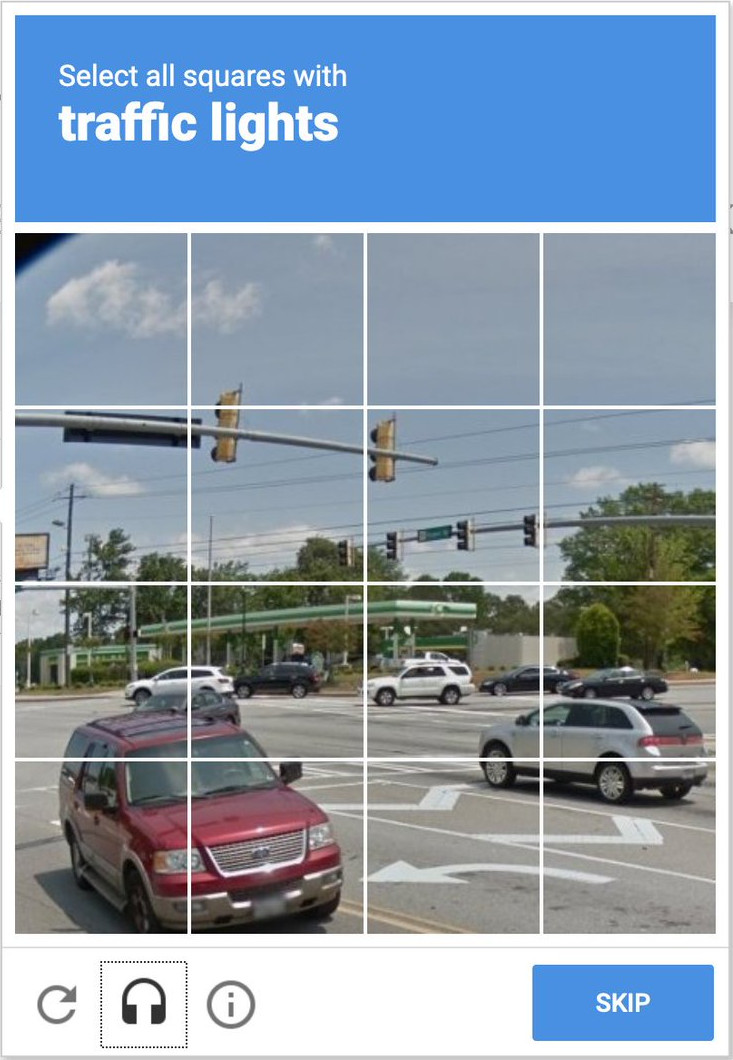
\includegraphics[width=.68\linewidth]{Images/StateOfArt/selection_CAPTCHA}
         \caption{\footnotesize{With an image divided in sub-squares.}}
         \label{soa:selection}
     \end{subfigure}
     \hfill
     \begin{subfigure}[b]{0.48\textwidth}
         \centering
         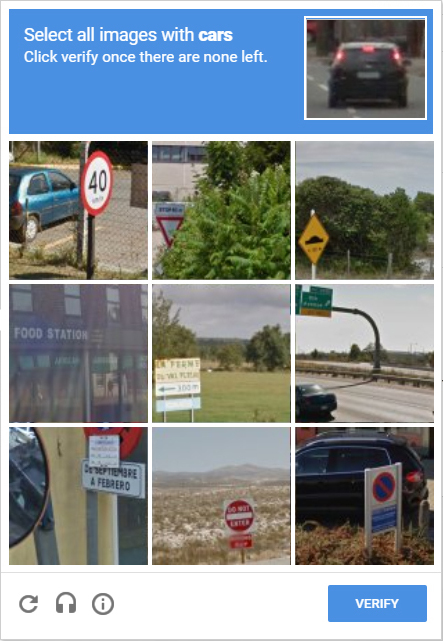
\includegraphics[width=.68\linewidth]{Images/StateOfArt/selection_CAPTCHA2}
         \caption{\footnotesize{With several images.}}
        \label{soa:selection2}
     \end{subfigure}
     \caption{\footnotesize{Examples of selection-based CAPTCHAs.}}
\end{figure}
}
\descItem{Interactive-based CAPTCHAs}
{the user needs to discover a secret position in an image using mouse movements or swiping gestures
\begin{figure}[h]
     \centering
     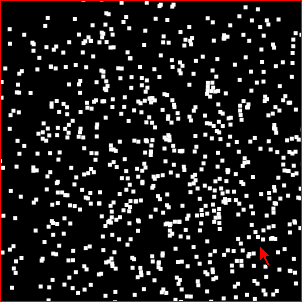
\includegraphics[width=.4\linewidth]{Images/StateOfArt/interactive_CAPTCHA}
     \caption{\footnotesize{Example of interactive-based CAPTCHA.}}\label{soa:interactive_CAPTCHA}
\end{figure}
}
\end{itemize}

\subsection{Math CAPTCHAs}
Looking to a math operation, specified in a frame, the user needs to insert the result in a text field. The operation is written in plain text or, to improve the security of this challenge, it's warped like text-based CAPTCHAs (see \myref{Figure}{soa:arithmetic}). These classical math-CAPTCHAs, also known as \textit{arithmetic CAPTCHAs}, are vulnerable to OCR (Optical Character Recognition) techniques.\\
\begin{figure}[h]
     \centering
     \begin{subfigure}[b]{0.48\textwidth}
         \centering
         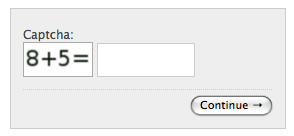
\includegraphics[width=.7\linewidth]{Images/StateOfArt/math_CAPTCHA}
         \caption{\footnotesize{With plain text.}}
     \end{subfigure}
     \hfill
     \begin{subfigure}[b]{0.48\textwidth}
         \centering
         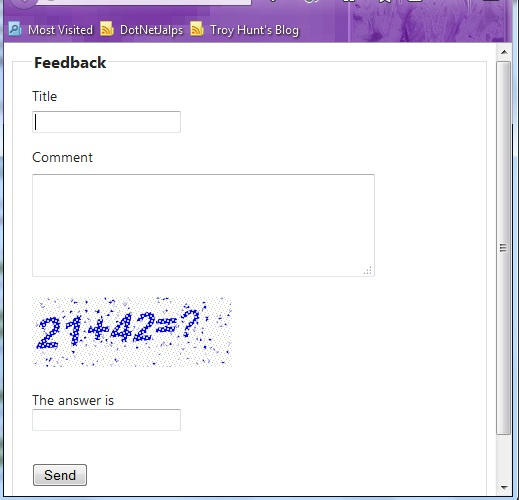
\includegraphics[width=.7\textwidth]{Images/StateOfArt/math_CAPTCHA2}
         \caption{\footnotesize{With wrapped text.}}
     \end{subfigure}
		\caption{\footnotesize{Example of arithmetic CAPTCHAs.}}
		\label{soa:arithmetic}
\end{figure}
An advanced version of this CAPTCHA is used in the Quantum Random Bit Generator Service (QRBGS) sign-up Web Page\cite{math_CAPTCHA} (see \myref{Figure}{soa:QRBGS}). This type of CAPTCHA asks the user to solve an advanced math expression. It prevents the use of free or commercial OCR techniques because many mathematical symbols are not considered in the traditional detection algorithms. Hence many math symbols are wrongly translated by bot programs and the challenge is very secure. However, this CAPTCHA is vulnerable to side-channel attacks \cite{math_CAPTCHA} and it's very complex for normal users. In fact many people can't solve it correctly because the required level of math knowledge is very high and not very common.
\begin{figure}[h]
     \centering
     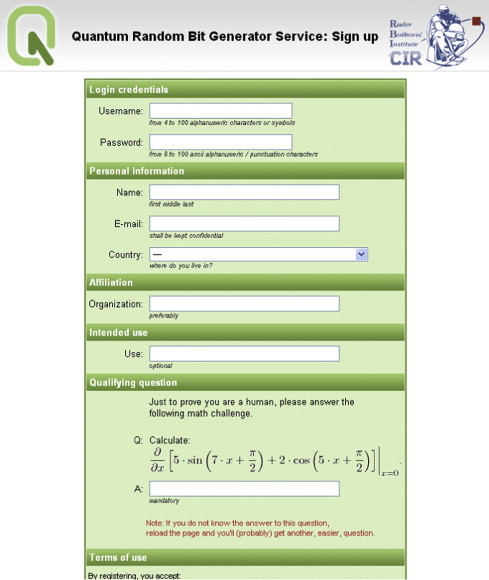
\includegraphics[width=.4\linewidth]{Images/StateOfArt/QRBGS}
     \caption{\footnotesize{Example of Quantum Random Bit Generator Service (QRBGS) sign-up Web Page \cite{math_CAPTCHA}.}}\label{soa:QRBGS}
\end{figure}

\subsection{Slider CAPTCHAs}
Slider CAPTCHAs ask users to move a slider across the screen. The image recognition is not part of the challenge.\\
The most popular CAPTCHAs of this type are the following:
\begin{itemize}
\descItem{CAPTCHA used by Taobao.com}{it asks the user to drag the slider from the start to the end of the sliding bar to verify his identity (see \myref{Figure}{soa:slider}).}
\descItem{CAPTCHA used by TheyMakeApps.com}{it asks the user to move the slider to the end of the line to submit a form\cite{sliding_CAPTCHA} (see \myref{Figure}{soa:slider2}).}
\end{itemize}
Over the years several implementations of this type of CAPTCHAs have been bypassed with a simple JavaScript code and puppeteer.
\begin{figure}[h]
     \centering
     \begin{subfigure}[b]{0.48\textwidth}
         \centering
         
\includegraphics[width=.8\linewidth]{Images/StateOfArt/taobao_CAPTCHA}
                  \caption{\footnotesize{Example of TaoBao.com CAPTCHA.}}
         \label{soa:slider}
     \end{subfigure}
     \hfill
     \begin{subfigure}[b]{0.48\textwidth}
         \centering
         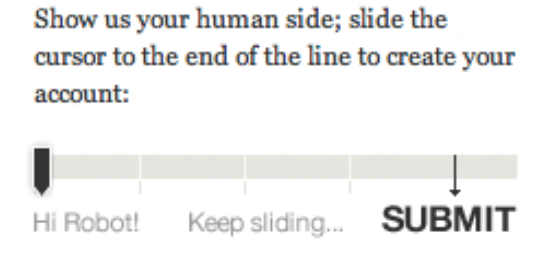
\includegraphics[width=.8\linewidth]{Images/StateOfArt/theyMakeApps_CAPTCHA}
         \caption{\footnotesize{Example of TheyMakeApps.com CAPTCHA.}}
        \label{soa:slider2}
     \end{subfigure}
     \caption{\footnotesize{Examples of slider CAPTCHAs.}}
\end{figure}

\subsection{Text-based CAPTCHAs}
In text-based CAPTCHA schemes a random series of warped characters and/or numbers is displayed on the screen inside an image (see \myref{Figure}{soa:text_CAPTCHA}). The user needs to understand which are the characters that composes the sequence and then he types them inside a text-field. The most known classes of text-based CAPTCHAs are:
\begin{itemize}
\descItem{2D}{the warped characters of the text are placed and oriented in a 2D plane, parallel to the screen plane. The image of the 2D plane is used in the challenge.}
\descItem{3D}{each warped character of the text is mapped into a 3D model of the character and then is placed and oriented in a 3D plane in the space. A 2D image of the 3D space is taken from a specific point of view and it's used in the challenge.}
\end{itemize}
This type of CAPTCHAs is vulnerable to several attacks, related to Computer Vision techniques:
\begin{itemize}
\item{OCR techniques\cite{OCR}}
\item{Segmentation techniques (e.g. DECAPTCHA\cite{DECAPTCHA})}
\item{Machine Learning and Deep Learning techniques}
\end{itemize}
In the design phase of a text-based CAPTCHA there are many issues, related to Computer Vision attacks, to be considered. For each of them, there is usually a solution in the design phase of the CAPTCHA that reduces the probability that the challenge will be broken by a bot\cite{DECAPTCHA}.
\begin{figure}[h]
     \centering
     
\includegraphics[width=.55\linewidth]{Images/StateOfArt/text_CAPTCHA}
     \caption{\footnotesize{Example of text-based CAPTCHA.}}\label{soa:text_CAPTCHA}
\end{figure}

\subsection{Video-based CAPTCHAs}
This type of CAPTCHAs isn't very common because it requires the download of a very large file\cite{survey_advanced_CAPTCHA}. The traditional video-based CAPTCHA is composed by a video in which a sliding text is shown (see \myref{Figure}{soa:video}). The user needs to type this message in a text field to pass the challenge. Some implementations of this type of CAPTCHAs are vulnerable to machine learning attacks.\\
Another version of the CAPTCHA is \textit{Motion CAPTCHA}\cite{Motion_CAPTCHA}, developed by M. Shirali-shahreza and S. Shirali-shahreza, in which the user needs to watch a video. Then he needs to select which action was performed in the played file, choosing it from multiple answers (see \myref{Figure}{soa:video2}). The strength of these implementations of CAPTCHAs is in the relationship between the multiple choices of the answer\cite{video_attack}.\\
A similar implementation of the previous version is the one developed by Kluever et al. in which the user watches a video and then he needs to write three words that describe what he sees\cite{video_desc}. The same authors created a tag frequency-based attack to evaluate the security of their CAPTCHA scheme and they achieve a success rate of 13\%.
\begin{figure}[h]
     \centering
     \begin{subfigure}[b]{0.48\textwidth}
         \centering
         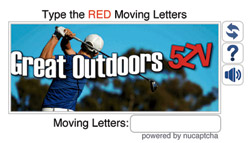
\includegraphics[width=\linewidth]{Images/StateOfArt/video_CAPTCHA}
         \caption{\footnotesize{Example of sliding text in video.}}
         \label{soa:video}
     \end{subfigure}
     \hfill
     \begin{subfigure}[b]{0.48\textwidth}
         \centering
         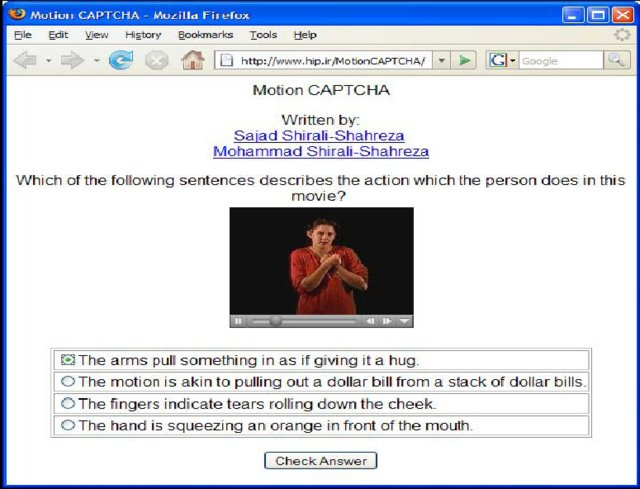
\includegraphics[width=\linewidth]{Images/StateOfArt/video_CAPTCHA2}
         \caption{\footnotesize{Example of Motion CAPTCHA\cite{Motion_CAPTCHA}.}}
        \label{soa:video2}
     \end{subfigure}
     \caption{\footnotesize{Examples of video-based CAPTCHAs.}}
\end{figure}

\section{Modern CAPTCHAs}
The type of CAPTCHAs and authentication mechanisms, described in the following sections, are different from traditional CAPTCHAs because they don't challenge the cognitive capabilities of a human user. They work leveraging other parameters, such as behavioural analysis and data of the sensors. In the following sections there is a summary of the most known CAPTCHA schemes of this type.

\subsection{Biometrics-based CAPTCHAs}\label{soa:Bio_CAPTCHA}
Biometric-based CAPTCHAs are very often used to support the authentication mechanisms of a user. The most known schemes of this type are the following:
\begin{itemize}
\descItem{Bio-CAPTCHA voice-based Authentication}
{This authentication method was developed starting from good results reached in the authentication phase of cloud systems\cite{voice_CAPTCHA} (Alexa for Amazon, Siri for Apple, Cortana for Microsoft). This particular implementation uses a random voice-based password challenge. This password changes at every login and the user needs to say it out loud. The strength of the challenge is the peculiarity of the human voice. The experiments reveals that unauthorized access probability decreases, while the usability is very high because it requires only the access to the microphone.}
\descItem{rtCAPTCHA}{this type of authentication method is a Real-time CAPTCHA that asks users to perform some tasks like smile, blink or nod in front of the camera of the mobile phone. The recorded video is sent to the service provider that checks if there is the expected user performing the required action in the file.\\
In the work of Erkam Uzun, Simon Pak Ho Chung, Irfan Essa and Wenke Lee\cite{rtCAPTCHA}, there is a detailed comparison between other similar authentication mechanisms and rtCAPTCHA, evaluating all possible Computer Vision attacks.}
\end{itemize}

\subsection{Behavioural-based CAPTCHAs}
In 2014 Google announced that the Artificial Intelligence can solve now even the most difficult variant of text-based CAPTCHAs at 99.8\% accuracy\cite{break_text}. For this reason, the company develops the following CAPTCHA schemes:
\begin{itemize}
\descItem{Google no CAPTCHA}
{Google developed this new CAPTCHA system in 2015. It's simpler than traditional CAPTCHAs in terms of user interaction\cite{google}. This CAPTCHA system is composed by two layers of protection:
\begin{enumerate}
\item{Checkbox \textit{"I'm not a robot"} to be clicked by the user as shown in \myref{Figure}{soa:noCAPTCHA} (or image-based CAPTCHA on mobile devices)
\begin{figure}[h]
     \centering
     
\includegraphics[width=.4\linewidth]{Images/StateOfArt/noCAPTCHA}
     \caption{\footnotesize{Example of Google no CAPTCHA checkbox.}}\label{soa:noCAPTCHA}
\end{figure}
}
\item{Traditional text-based CAPTCHA with two warped words}
\end{enumerate}
The second layer is reached only if the user doesn't succeed in the first one. For the checkbox step, the application evaluates in background the user's behaviour (e.g. the mouse movement, where the user clicks, how long he lingers over a checkbox). Then the program performs an \textit{advanced risk analysis}, by looking at the results of the first step, the spam traffic and the number of passed/failed challenges. In this way the CAPTCHA understands if the test is passed or not.\\
The experimental results confirm that the first phase is very inefficient and many times the user fails performing this challenge even if he was a human and was performing correctly the task. A problem of this type of CAPTCHA is that many attacks exploits the image-based CAPTCHA (used on mobile phones) and the text-based CAPTCHA of the second phase using attacks based on known Computer Vision techniques or their variants (e.g. CAPTCHA breaker made by Suphannee Sivakorn, Jason Polakis and Angelos D. Keromytis\cite{break_google}).
}
%HERE
\descItem{Google Invisible ReCAPTCHA}
{it's a top layer over the \textit{Google noCAPTCHA v2.0}. It adds the option to bind the CAPTCHA directly to the form’s submit element. In this way, the programmer can add layers to reduce the user experience of a bot\cite{google}. It usually requires the use of cookies to track the user's behaviour. There exist two version of this CAPTCHA:
\begin{itemize}
\descItem{ReCAPTCHA v2.0}
{it was developed in 2017. It's not really invisible because Privacy \& Policy badge must be included on every pages of an app or a website in which the CAPTCHA is used. Computer Vision and Artificial Intelligence algorithms can break the challenges by recognizing object in the pictures in the image-based CAPTCHA phase.}
\descItem{ReCAPTCHA v3.0}
{it was developed in 2018. It constantly analyses the human behavior, the mouse movements, the typing speed and the other features in NO CAPTCHA technology until Google collects enough data to tune their Google Invisible reCAPTCHA v2.0. This type of CAPTCHAs uses the probability scores of Artificial Intelligence and Machine Learning, the hostname, the timestamp and the action validation.\\
Google removes the image recognition phase and looking only at the score, it evaluates if the user is a human or a bot. The main difference with respect to the previous versions of Google modern CAPTCHAs is that it returns a probability score, called \textit{risk score}, in the range $[0.0, 1.0]$: \textit{0.0} if the user is a bot, \textit{1.0} otherwise. The administrator of the website can decide what range of scores he wants to manage, declaring when the site is under attack and what actions need to be performed.\\
Over the year, several peculiarities and problems of this version of \textit{Invisible ReCAPTCHA} were discovered. For example:
\begin{itemize}
\item{If a user accesses a Web page using incognito mode or private mode, he is classified with a very low score (\textit{high risk}).}
\item{If a human is wrongly classified as a bot, the user can login into its Google account to increase its score. If this doesn't change the classification, you cannot do anything else.}
\end{itemize}
}
\end{itemize}
}
\end{itemize}

\subsection{Sensor-based CAPTCHAs}
The devices, with access to the net, have natively many sensors nowadays, like the gyroscope and the accelerometer. The CAPTCHA schemes, described in the following sections, leverage the data generated from these sensors to improve the security of the authentication.
\begin{itemize}
\descItem{Completely Automated Public Physical test to tell Computer and Humans Apart (CAPPCHA)}
{this is a way to enforce the PIN authentication phase by mobile phone\cite{CAPPCHA}. The user needs to tilt the device to a specified angle, specified on the screen (see \myref{Figure}{soa:CAPPCHA}). The CAPPCHA security is based on the \textit{Secure Element} (\textit{SE}) in the device. It prevents brute force, side channel and recording attacks. The usability results are good because many comments, made by the users, were also considered in the implementation.
\begin{figure}[h]
     \centering
     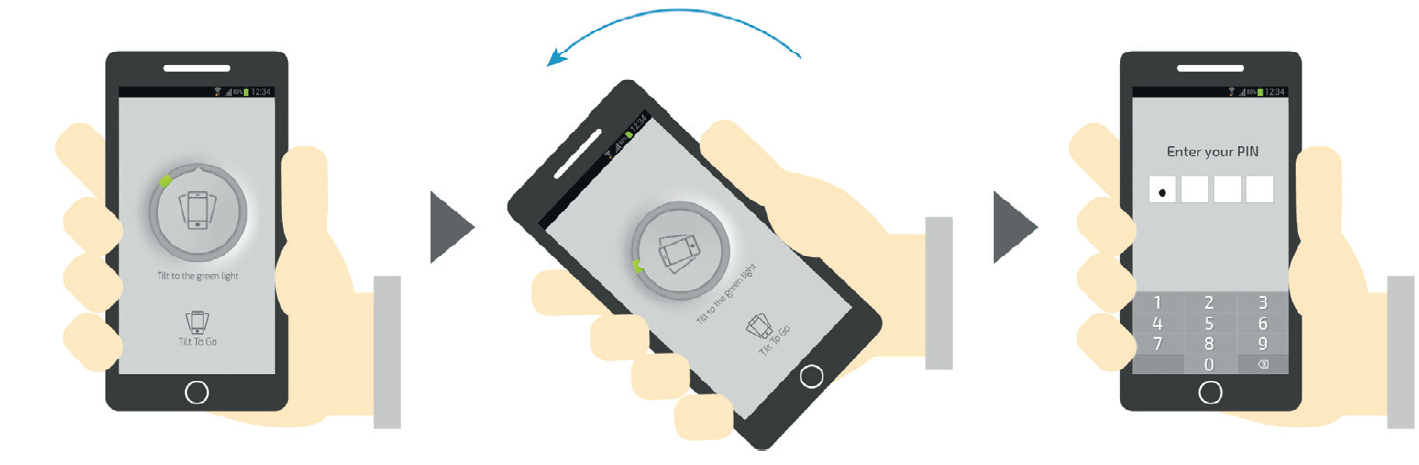
\includegraphics[width=.8\linewidth]{Images/StateOfArt/CAPPCHA}
     \caption{\footnotesize{CAPPCHA and PIN authentication\cite{CAPPCHA}.}}\label{soa:CAPPCHA}
\end{figure}
}
\descItem{Invisible CAPPCHA}
{It will be described in details in \myref{Chapter}{chapter:InvisibleCAPPCHA}.}
\end{itemize}

\section{CAPTCHA security}\label{soa:security_CAPTCHAs}
The process used to break many traditional CAPTCHAs, based on text or images, is usually organized into the following phases\cite{CAPTCHA_attack_process}:
\begin{enumerate}
\descItem{Pre-processing phase}
{in this phase, several techniques are applied to remove background, to separate foreground from the background, to delete noise and to remove some particular pattern (e.g. Canny Detection and Scale-Invariant Feature Transform (SIFT) application).
}
\descItem{Attack phase}
{the following techniques are usually applied:
\begin{itemize}
\descItem{\textit{Object recognition attacks}}
{The most used techniques are pattern matching (e.g. shape context matching, correlation algorithm), OCR recognition, SIFT and machine learning. They are usually applied after the segmentation of the image with several methods (e.g. vertical histogram, color filling, snake segmentation and JSEG).}
\descItem{\textit{Random Guess Attacks}}
{The attacker's program tries to break the CAPTCHA scheme by guessing the correct answer. This attack is effective on CAPTCHAs with few number of different challenges.}
\descItem{\textit{Human Solver Relay Attacks}}
{The bot forwards the CAPTCHA challenge to a remote human worker that will solve it if the previous phases don't produce good results. This technique is usually used also to solve other types of CAPTCHAs.}
\end{itemize}
}
\end{enumerate}
Many CAPTCHA schemes have still several issues:
\begin{itemize}
\descItem{Session issue}
{Some types of CAPTCHAs have a big issue because they don't destroy the session, after a correct answer is inserted by the user\cite{text_audio}.\\
Hence, the hacker can crack the next accesses using the same session id with the related solution of the challenge, after connecting to the web page of CAPTCHA. In this way the attacker can make hundreds of requests before the session expires and the previous operation must be computed again.}
\descItem{Resilience to both automated and human solver relay attacks}
{Many CAPTCHA schemes are designed to be robust against a possible AI attack but the new generation of CAPTCHAs involves the use of remote bot or human solver. Traditional CAPTCHA schemes are vulnerable to this type of attacks.\\
Sensor-based CAPTCHAs are often vulnerable to relay attacks. An exception is the \textit{Invisible CAPPCHA}, that will be analysed in \myref{Chapter}{chapter:InvisibleCAPPCHA}.
}
\descItem{Limited number of challenges}
{An issue of sensor-based CAPTCHA schemes is the limited number of challenges because the design of many usable gestures is very hard. This problem could be solved
relying on trusted hardware.}
\descItem{Trade-off between Friction-heavy and Frictionless CAPTCHAs}
{A trade-off between usability and security aspects is always considered analysing CAPTCHA schemes. This condition is exacerbated in behavioural and sensor-based CAPTCHAs.}
\descItem{User's privacy}
{Sensor-based and behavioural CAPTCHAs usually send useful information to a remote server that analyses it to establish if the user was a human or a bot. If an hacker attacks the server side of this application, he can access users' private data.\\
In some CAPTCHAs, the information is evaluated on the client side by a trusted hardware and the server receives only the results of the analysis. In this case, we need to be sure that trusted hardware is secure enough to guarantee privacy of user's information.
}
\descItem{Compatibility with different devices}
{Many CAPTCHA schemes, e.g. behavioural ones, use specific forms factors but a good challenge should be compatible with different factors.}
\end{itemize}

\begin{sidewaystable}
\centering \footnotesize
\renewcommand*\arraystretch{1.3}
\begin{tabular}{ccll}
\toprule
\multicolumn{1}{c}{\textbf{Type}} & \multicolumn{1}{c}{\textbf{Scheme}} & \multicolumn{1}{c}{\textbf{Usability issues}} & \multicolumn{1}{c}{\textbf{Security}}\\
\midrule
%Audio row
\multirow{3}{*}{\textbf{\textit{Audio}}} & {\textit{Audio reCAPTCHA}} & {Issues of recognition:} & {It's vulnerable to:}\\
&&{\itemCell{Knowledge of English dictionary by the user.}}&{\itemCell{ASR programs.}}\\
&&{\itemCell{Some character sounds very similar to others.}}&{\itemCell{Deep Learning and ML techniques.}}\\
\midrule
\multirow{2}{*}{\textbf{\textit{Game}}} & {\textit{Dynamic Cognitive}} & {Comprehension of rules.} & {Vulnerable to Stream Relay Attack}\\
& {\textit{Game (DCG)}} &&\\
\midrule
\multirow{5}{*}{\textbf{\textit{Image}}} & {\textit{Click-based}} & {Difficulty in identification of images caused by:} & {Vulnerable to:}\\
& {\textit{Drag \& Drop-based}} & {\itemCell{Blur of images.}} & {\itemCell{Segmentation techniques}}\\
& {\textit{Sliding-based}} & {\itemCell{Low vision condition.}} & {\itemCell{Deep Learning and ML techniques}}\\
& {\textit{Selection-based}} && {OCR techniques}\\
& {\textit{Interactive-based}} &&\\
\midrule
%Math row
\multirow{3}{*}{\textbf{\textit{Math}}} & {\textit{Arithmetic}} & {It requires basic or advanced} & {Vulnerable to:}\\
{} & {\textit{QRBGS}} & {math knowledge.} & {\itemCell{OCR techniques}}\\
&&&{\itemCell{Side-channel attacks}}\\
\midrule
\multirow{2}{*}{\textbf{\textit{Slider}}} & {Taobao.com} & {Simple and intuitive interaction} & {Simple bypassed by Javascript code}\\
& {TheyMakeApps.com} & {} & {and pupeeteer}\\
\midrule
\multirow{5}{*}{\textbf{\textit{Text}}} & {\textit{2D}} & {Many problems have to be solved by user:} & {It can be identified by:}\\
&{\textit{3D}}&{\itemCell{Multiple fonts}}&{\itemCell{OCR technique}}\\
&&{\itemCell{Font size}}&{\itemCell{Segmentation techniques}}\\
&&{\itemCell{Blurred Letters}}&{\itemCell{Deep Learning and ML techniques}}\\
&&{\itemCell{Wave Motion}}&\\
\midrule
{\textbf{\textit{Video}}} & {\textit{Motion CAPTCHA}} & {Heavy file to be downloaded} & {}\\
\bottomrule
\end{tabular}
\caption{\footnotesize{Survey of main types of traditional CAPTCHAs\cite{survey_CAPTCHA}.}}
\label{soa:traditional_table}
\end{sidewaystable}

\begin{comment}
\begin{sidewaystable}
\centering \footnotesize
\renewcommand*\arraystretch{1.3}
\begin{tabular}{ccll}
\toprule
\multicolumn{1}{c}{\textbf{Alternative Type}} & \multicolumn{1}{c}{\textbf{Name of implementation}} & \multicolumn{1}{c}{\textbf{Usability issues}} & \multicolumn{1}{c}{\textbf{Security}}\\
\midrule
\textit{} & {} & {}\\
\bottomrule
\end{tabular}
\caption{\footnotesize{Survey of main types of alternatives of CAPTCHAs\cite{survey_CAPTCHA}.}}
\label{soa:modern_table}
\end{sidewaystable}
\end{comment}
\chapter{Invisible CAPPCHA}\label{chapter:InvisibleCAPPCHA}
The \textit{Invisible CAPPCHA} is an evolution of CAPPCHA, in terms of usability\cite{Invisible_CAPPCHA}. The main difference with respect to CAPPCHA is that the challenge is not explicitly submitted to the user but it is embedded in the PIN authentication phase leveraging a side channel. Invisible CAPPCHA works only on smartphones as its ancestor but it's very important to understand how data, obtained by the sensors, could be leveraged during the authentication phase.\\
Invisible CAPPCHA is a method developed in 2018 and based on motion side-channel of mobile devices and it's very effective as support to Password-based authentication methods. The main steps, followed by this CAPTCHA, are:
\begin{enumerate}
\descItem{Motion detection}{in this phase the micro-movements of the device, generated by the interaction of the user with the touch-screen, are evaluated by the \textit{Secure Element} (\textit{SE})}
\descItem{Communication between Client and Server}{in this phase the credentials are shared with the remote Service Provider}
\end{enumerate}
The following sections will analyse this steps highlighting some peculiarities of Invisible CAPPCHA that will be used or modified to develop AcCAPPCHA, a CAPTCHA based on microphone sensors.

\section{Motion detection}
In this first phase, Invisible CAPPCHA exploits the accelerometer of the mobile device. It detects the acceleration over the three axis in g-force units, as a sequence of vectors over time:
$$\{ A_i\}_{i=1}^{n} = \{ (a_1^x, a_1^y, a_1^z), ..., (a_n^x, a_n^y, a_n^z)\}$$
This type of side-channel information from embedded accelerometer has been exploited in different attacks for the single and double tap detection. These attacks analyse the accelerations over the z-axis by comparing them to some thresholds and some timing conditions.\\
In Invisible CAPPCHA, the side-channel information is stored on the memory of the mobile device. Depending on the device, a smartphone built-in vibration can be generated along Z axis or along more than one axis (see \myref{Figure}{inv:vibration}). On the contrary a finger tap event is defined by strong accelerations on Z-axis but also similar one to the other (see \myref{Figure}{inv:tap}).\\
In Invisible CAPPCHA, the difference between built-in vibration and tap acceleration is evaluated by a simple algorithm. It relies on negative and positive peaks, that are detected by comparing acceleration along Z axis with predefined thresholds. The differences between the tap accelerations and the vibrations is the main characteristic that guarantees user's tap cannot be simulated by a bot using the vibration motors.\\
Another important requirement, to prevent a bot attack, is that Invisible CAPPCHA uses a Secure Element that embedded the accelerometer of the device. In this way malicious code can't access to the sensor. Nowadays there exists a smart card, called SIMSense, that already integrates motion sensor and embeds it in a Secure Element.\\
\begin{figure}[h]
     \centering
     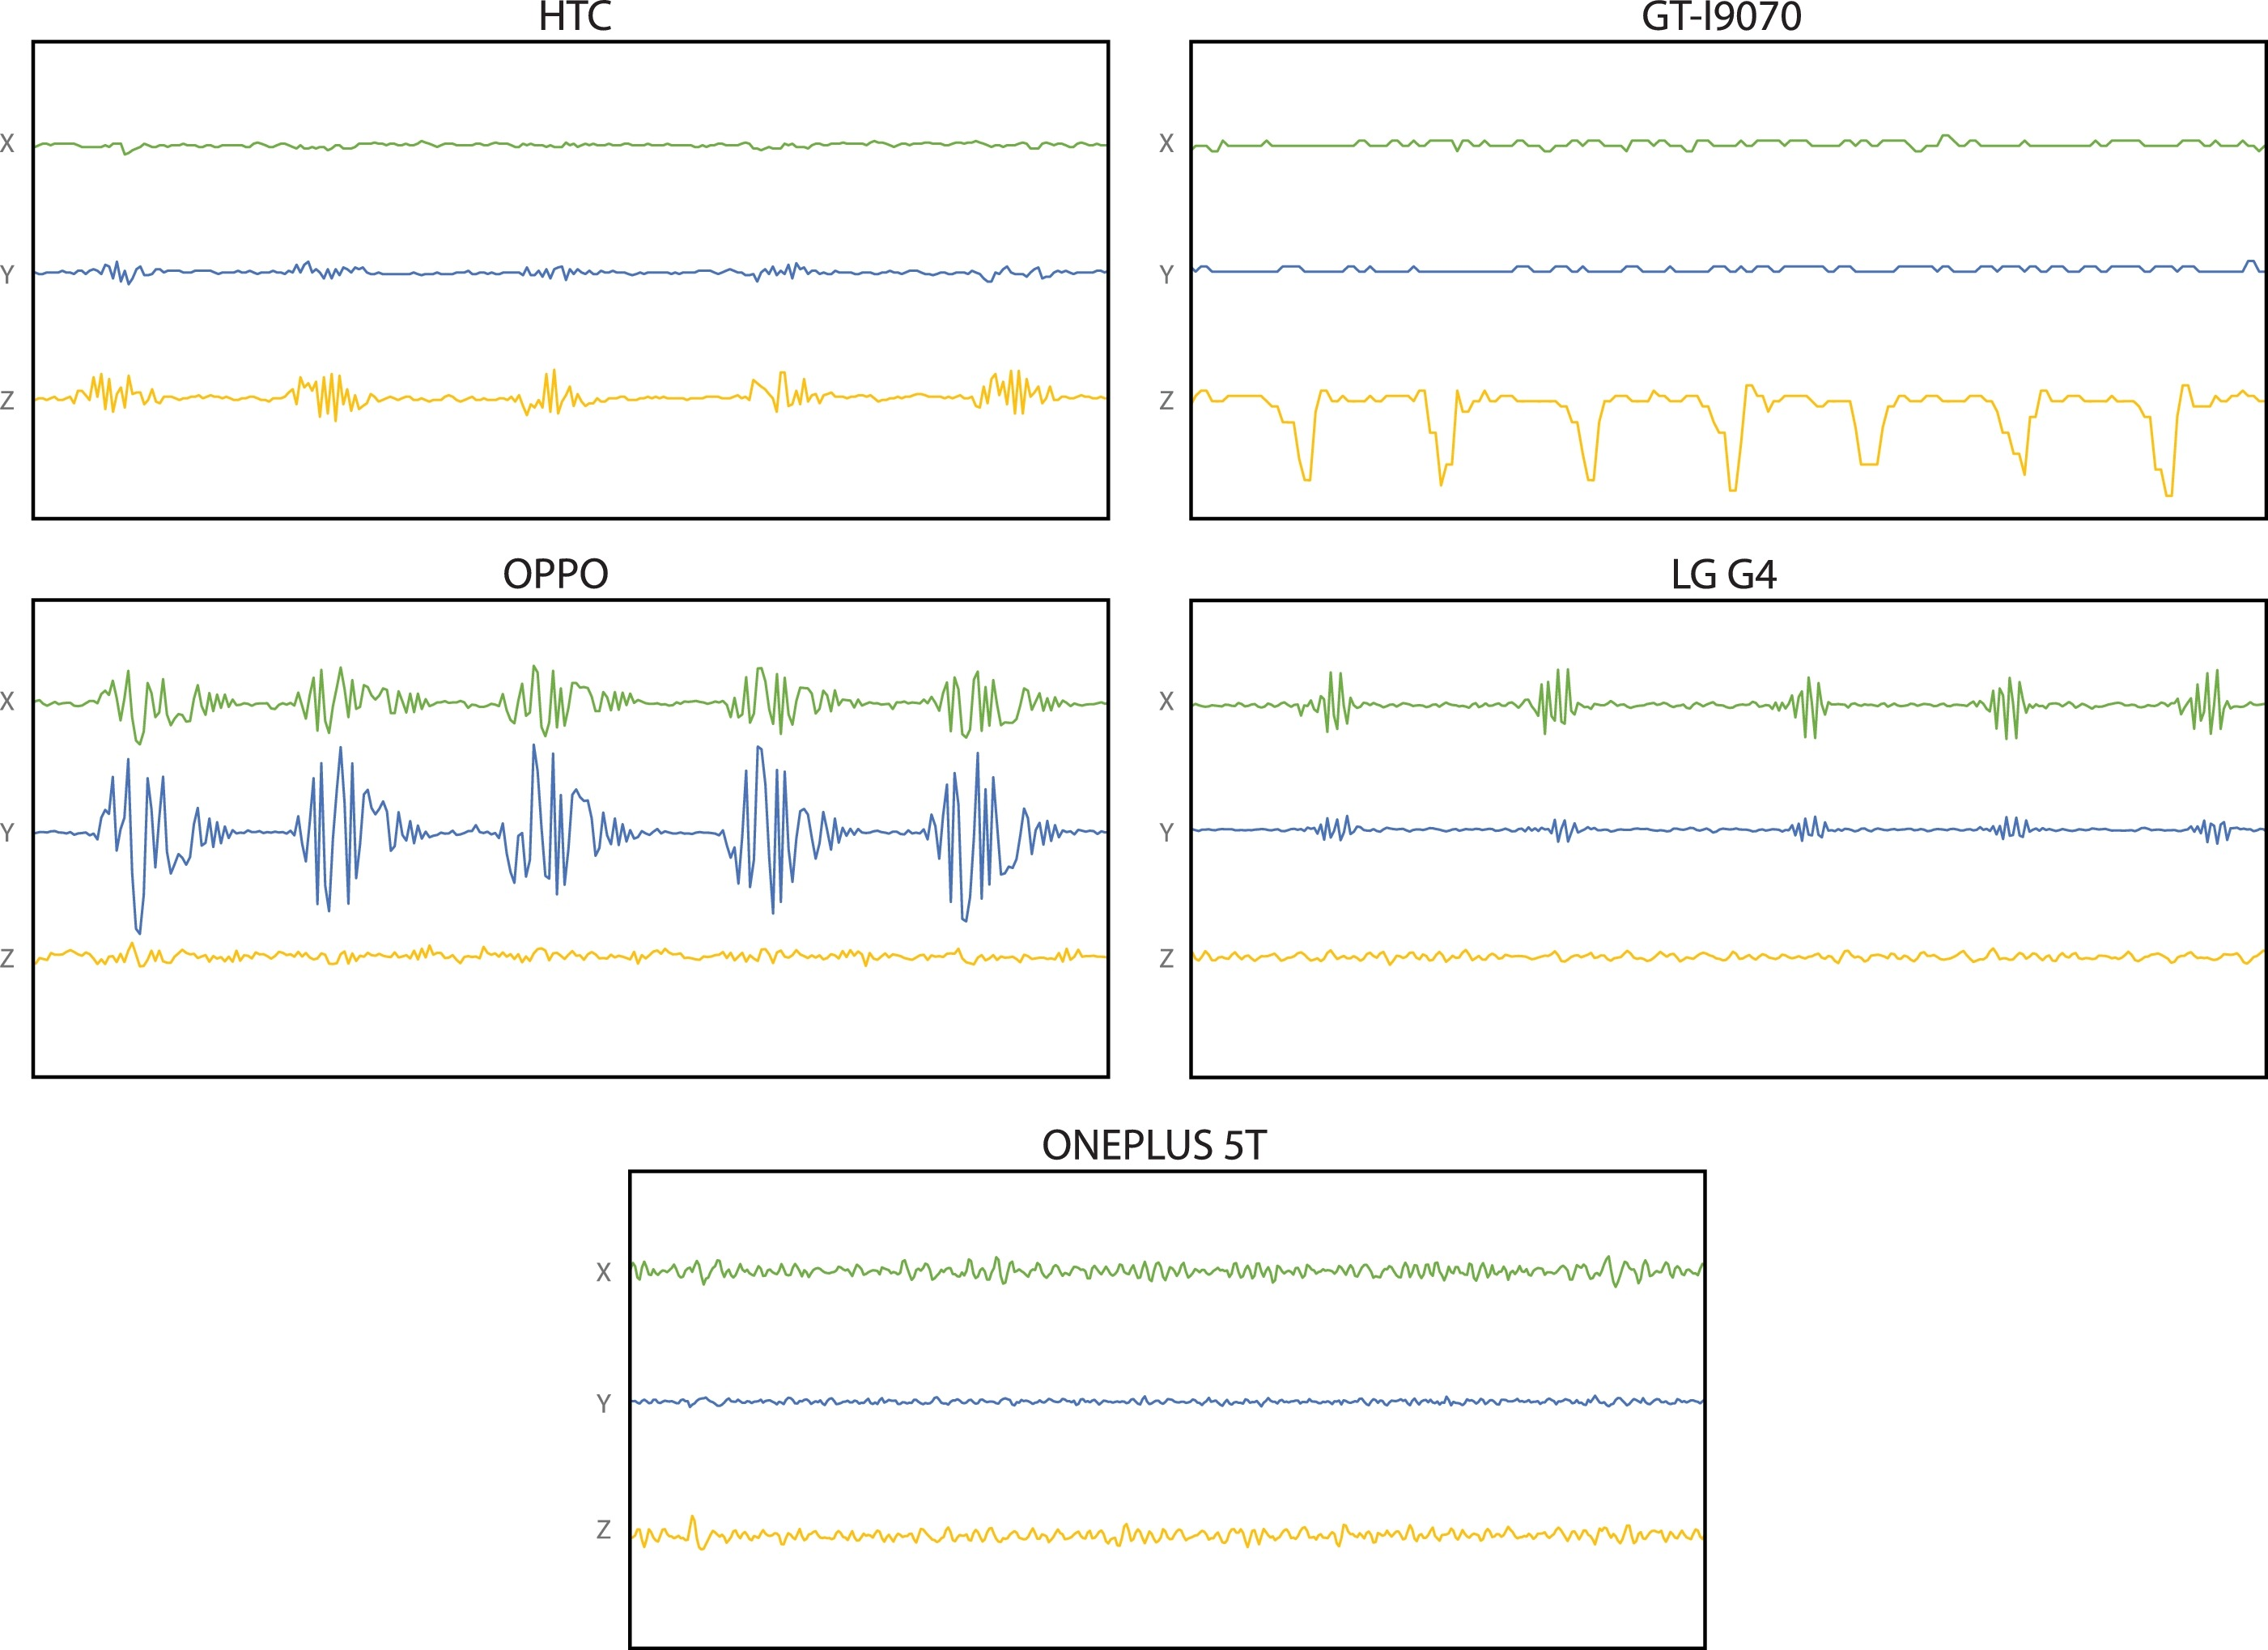
\includegraphics[width=.8\linewidth]{Images/InvisibleCAPPCHA/vibration}
     \caption{\footnotesize{Example of accelerations caused by smartphone built-in vibration.}}\label{inv:vibration}
\end{figure}
\begin{figure}[h]
     \centering
     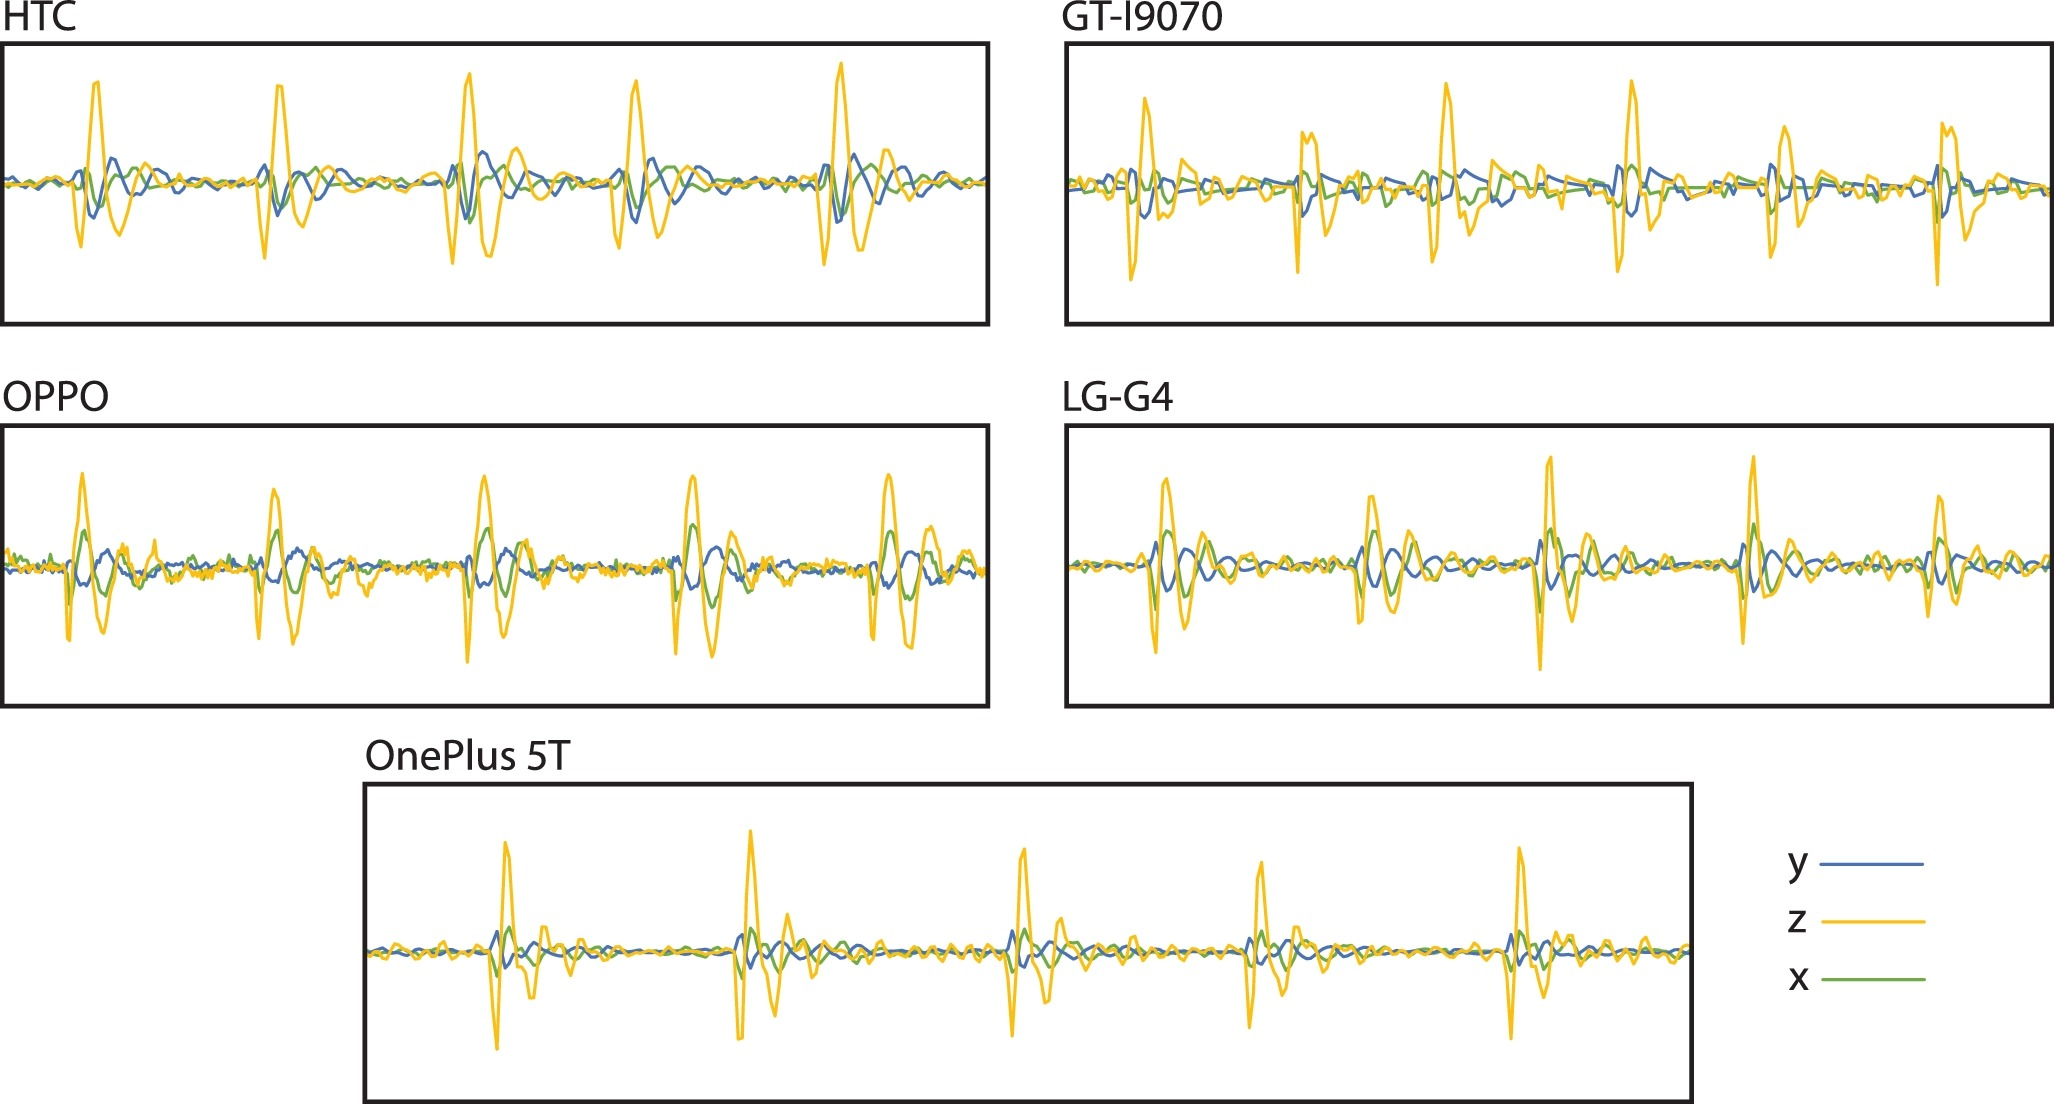
\includegraphics[width=.8\linewidth]{Images/InvisibleCAPPCHA/tap}
     \caption{\footnotesize{Example of accelerations caused by finger tap detection.}}\label{inv:tap}
\end{figure}


\section{Communication between Client and Server}\label{inv:communication}
When the user fills a form or provides other information to a cloud application/service, the Secure Element checks if a micro-movement is measured when a user tap is detect. If this happens the input inserted by user is considered valid, or rather generated by a human, otherwise the algorithm tells that the input was generated by a bot.\\
An extra message, that tells if the task was performed by a user or not, is sent to the server side. The integrity of this message is guaranteed by the Secure Element, that can be equipped with a digital signature. The identity of the device can be associated to the message sent and then it can be checked and verified. The Secure Element signs the verification message through ECDSA.

\subsection{Elliptic Curve Digital Signature Algorithm (ECDSA)}
The elliptic cryptography works similarly to RSA but it uses smaller keys. The signature algorithm with elliptic curves is divided in two phases, like the one based on RSA. Considering two users, Alice and Bob, ECDSA phases are explained in the following lines:
\begin{itemize}
\descItem{Sign generation}
{If Alice wants to send a message, protected with digital sign, to Bob, they need to share the following parameters \textit{(curve, G, n)}: \textit{curve} is the equation of an elliptic curve, \textit{G} is the base point of prime order on the curve and \textit{n} is the multiplicative order of \textit{G} for which $n\; x\; G = O$ ($x$ is the scalar multiplication of a point of the curve).
Alice generates a private key $d_A$ in the range $[1, n-1]$ and a public key $Q_A=d_A\; x\; G$. Alice needs to perform \myref{Algorithm}{inv:ECDSA_sign} to sign a message $m$.
\begin{algorithm}[h]
\DontPrintSemicolon\footnotesize
\KwIn {$\mathtt{m}$= message to be signed}
\KwOut {$\mathtt{(r,s)}$= digital sign}
\BlankLine
$e\gets HASH(m)\;$where \textit{HASH} is an hash function (e.g. SHA-2)\;
\BlankLine
$z \gets$ string composed by the $L_n$ most left bits\;
$\;\;\;\;\;\;\;$where $L_n$ is the bit length of the group of order $n$\;
$r\gets 0$\;
$s\gets 0$\;
\BlankLine
\While{$r=0\;mod\;n$ or $r=0\;mod\;n$}{
	\BlankLine
	$k\gets RANDOM([1,n-1])$\;
	\BlankLine
	$(x_1, y_1)=k\;x\;G$ of the elliptic curve\;
	\BlankLine
	$r\gets x_1\; mod\; n$\;
	\BlankLine
	{$s\gets k^{-1}(z+rd_{A})\; mod\; n$}
	\BlankLine
}
\caption{Sign generation.}\label{inv:ECDSA_sign}
\end{algorithm}
}
\descItem{Sign verification}
{Bob wants to verify the digital signature sent by Alice. To do it, he needs to apply in order \myref{Algorithm}{inv:ECDSA_key_verify} and \textbf{\ref{inv:ECDSA_verify}}.\\
\begin{algorithm}[h]
\DontPrintSemicolon\footnotesize
\KwIn {$\mathtt{Q_A}$= public key to be verified}
\KwOut {$\mathtt{check}$= true if public key is correct}
\BlankLine
$\mathtt{check}\gets true$\;
\BlankLine
$\setminus\setminus$Valid coordinates\;
\If{$Q_A=O$}
{	
$\mathtt{check}\gets false$\;
}
\BlankLine
$\setminus\setminus$Element of the curve\;
\If{$Q_A\;\in$ curve}
{	
$\mathtt{check}\gets false$\;
}
\BlankLine
$\setminus\setminus$Correctness of order\;
\If{not $n\;x\;Q_A=O$}
{	
$\mathtt{check}\gets false$\;
}
\caption{Verification that public key is on the elliptic curve.}\label{inv:ECDSA_key_verify}
\end{algorithm}
\begin{algorithm}[h]
\DontPrintSemicolon\footnotesize
\KwIn {$\mathtt{(r,s,m)}$= digital sign and message}
\KwOut {$\mathtt{m}$= message to be signed}
\BlankLine
$e\gets HASH(m)\;$where \textit{HASH} is an hash function (e.g. SHA-2)\;
\BlankLine
$z \gets$ string composed by the $L_n$ most left bits\;
where $L_n$ is the bit length of the group of order $n$\;
\BlankLine
\If{not $r\;\in [1, n-1]$ or not $s\;\in [1, n-1]$}
{*Invalid sign*}
$e\gets HASH(m)\;$\;
\BlankLine$z \gets$ string composed by the $L_n$ most left bits\;
$w=s^{-1}\; mod\; n$\;
\BlankLine
$u_1 =zw\; mod\; n$\;
$u_2 =rw\; mod\; n$\;
$(x_1, y_1)=u_1\; x\; G\;+\; u_2\; x\; Q_{A}$ of the elliptic curve\;
\BlankLine
\If{$r\equiv x_1\; (mod\; n)$}
{*Verified sign*}
\Else{*Not accepted sign*}
\BlankLine
\caption{Sign verification.}\label{inv:ECDSA_verify}
\end{algorithm}
}
\end{itemize}
In Invisible CAPPCHA the message \textit{m} is bitwise concatenated with a signed unique value, the nonce \textit{n}, and then the signature is computed on their concatenation, $m||n$. Hence the signed message sent to the server is $(r, s, m, n)$.

\section{Security analysis}
After the verification of the signature, the communication must be also encrypted to ensure integrity and authenticity of exchanged messages.\\
The Secure Element can be accessed only through PIN authentication of the off-card communication party. If the malicious code has enough privileges to access Secure Element, some popular attacks can't be performed by an attacker.\\

\subsection{Strength against popular attacks}\label{inv:attacks}
The most popular attacks, that have been analysed, are\cite{Invisible_CAPPCHA}:
\begin{itemize}
\descItem{Replay attack}
{Because the message is signed together with a nonce, an attacker can't easily use a message already sent by a client to the server. In fact, the server checks if a nonce was already used by the client and if so, the server refuse the message sent by the attacker.
}
\descItem{Reverse engineering attack}
{Even if the attacker can de-obfuscate the code of the application running on the browser, he can access to reserved data on the server only if the verification message for human interaction was correctly signed by the Secure Element. Hence this type of attack can't be performed.}
\descItem{Human-solver relay attack}
{The Invisible CAPPCHA is strong to this type of attack because it doesn't require any additional task to be sent to a remote human solver, as in standard CAPTCHAs.}
\descItem{Brute force and password replay attacks}
{Invisible CAPPCHA can be used to validate every input before it is considered as a possible attempt for a password. If the password was inserted by a malware or was wrong, the number of attempts decreases. Hence this approach prevents a brute force attack. This also prevents the access to the Secure Element by the attacker in replay attacks.
}
\descItem{Denial Of Service (DOS)}
{If a malware tried more than the maximum amount of attempts of passwords it could do a Denial Of Service (DOS) of the Secure Element. To prevent this attack, the Secure Element can block access to itself if three invalid passwords are inserted by a human or if an invalid password is inserted by a bot.}
\end{itemize}
\begin{thebibliography}{9}
\bibitem{DECAPTCHA} E. Bursztein, M. Martin, and J. Mitchell, "Text-based CAPTCHA strengths and weaknesses" in \emph{Proc. 18th ACM Conf. Comput. Commun. Secur. (CCS), 2011, pp. 125–138.}

\bibitem{Improved_AUDIO} Jennifer Tam, Jiri Simsa, David Huggins-Daines, Luis von Ahn, and Manuel Blum, "Improving Audio CAPTCHAs" in \emph{Symposium On Usable Privacy and Security (SOUPS), 2008.}

\bibitem{TEXT_AUDIO} Sarika Choudhary, Ritika Saroha, Yatan Dahiya, and Sachin Choudhary, "Understanding CAPTCHA: Text and Audio Based Captcha with its Applications" in \emph{International Journal of Advanced Research in Computer Science and Software Engineering vol. 3 (6), pp. 106-115, June-2013.}

\end{thebibliography}
\chapter*{Acknowledgements}
Professor Migliardi\\\\
I would like to express my very great appreciation to Dr Guerar\\\\
I would like to express my gratitude to University of Padova for the study path I performed. The uncertainty about the future and the idea of being far from needed cyber security skills have become a stimulus to improve myself. I learn a lot and I got hooked on the programming, starting from zero level of it, thanks to the professors' professionalism and knowledge. During the last five years, I've changed and now I spend programming all my free time. Thanks to University because professors follow my thirst of knowledge and I grew up, living alone and really becoming an adult.\\\\
Thanks to staff,\\\\
Thanks to other company,\\\\
I would like to express my gratitude to my family that taught me to never give up. In particular thank to my sister that, with her great experience in University course, has been a reference for my study attitude and perseverance.\\\\
Thanks to my grandmother Concetta that, with her smiles, has left to me happiness during my darker and difficult periods.\\\\
Thanks to my grandmother Maria that, was always worried for my health issues and tries always to give me up using her food. \\\\
Thanks to Cristina,\\\\
Thanks to Francesca, because even if we had many commitments we have always found 5 minutes to stay together and to support the other one in his/her choices.\\\\
Thanks to Davide,\\\\
Thanks to Giuseppe, Aurora, Alessia and Sara,\\\\
Thanks to Elia,\\\\
Thanks to Lorenzo,\\\\

\end{document}